\documentclass[final,hyperref={pdfpagelabels=false}]{beamer}
%%% THEME FOR THE POSTER %%%
\usetheme{LTS5}

%%% PACKAGES DECLARATION
%%%%%%%%%%%%%%%%%%%%%%%%%%%%%%%%%%%%%%%%%%%%%%%%%%%
% Signal Processing Laboratory (LTS5) - EPFL      %
% LaTeX beamposter template                       %
% Authors:                                        %
%   D. Perdios – dimitris.perdios@epfl.ch         %
%   A. Besson – adrien.besson@epfl.ch             %
% v0.1 - 08.05.17                                 %
% Typeset configuration: pdfLaTeX + Biber         %
%%%%%%%%%%%%%%%%%%%%%%%%%%%%%%%%%%%%%%%%%%%%%%%%%%%

% Poster related package
\usepackage[orientation=portrait,size=a0,scale=1.4]{beamerposter} % Use the beamerposter package for laying out the poster with a portrait orientation and an a0 paper size
\usepackage{textpos}

% Typesetting
\usepackage[T1]{fontenc}
\usepackage[utf8]{inputenc}
\usepackage[english]{babel}
\usepackage{lmodern} % latin modern font
\usepackage{exscale} % scaling extension of the math fonts
%\usepackage[scaled]{helvet} % sans serif typo
\usepackage{csquotes} % pro­vides ad­vanced fa­cil­i­ties for in­line and dis­play quo­ta­tions (better to load when using biblatex)
\usepackage{textcomp} % pro­vide many text sym­bols (such as baht, bul­let, copy­right, mu­si­cal­note, onequar­ter, sec­tion, and yen), in the TS1 en­cod­ing
%\usepackage{setspace}
%	\onehalfspacing % 1.5 linespaceing (already in CLS)
%\usepackage{fancyhdr} % pro­vides ex­ten­sive fa­cil­i­ties, both for con­struct­ing head­ers and foot­ers, and for con­trol­ling their use
\usepackage{siunitx} % SI units system typset
%\usepackage{enumitem}
%	\setlist[enumerate]{label*=\arabic*.,topsep=5pt,partopsep=0pt,parsep=0pt,itemsep=2pt}
%	\setlist[itemize]{topsep=5pt,partopsep=0pt,parsep=0pt,itemsep=2pt}
\usepackage{fontawesome} % high quality web icons

% Math
\usepackage{amsmath}
\usepackage{amsfonts}
\usepackage{amssymb}
\usepackage{amsthm}
\usepackage{bm}
\usepackage{mathdots} % mathfonts for vdots
%\usefonttheme[onlymath]{serif} % uncomment for serif math equations

% Figures
\usepackage{graphicx}
	\graphicspath{{figures/}}
\usepackage{xcolor}
\usepackage[font=small, labelfont=bf, format=plain, labelsep=space, figurename=Figure, tablename=Table]{caption}
\usepackage[labelfont=sf, labelformat=parens, labelsep=space]{subcaption}

% Tables
%\usepackage{multirow}
\usepackage{longtable} % use \linebreak instead of \\ in headers to avoid a bug with longtables (or longtabu) across two pages
\usepackage{booktabs} % the pack­age en­hances the qual­ity of ta­bles (toprule, bottomrule, etc.)
\usepackage{tabu}
%	\renewcommand{\arraystretch}{1.3}

% Codes
\usepackage{listings}
%	Some style definitions
\lstdefinestyle{lstLaTeX}{
	aboveskip=0pt,
	belowskip=0pt,
    language=[LaTeX]TeX,
    breaklines=true,
    basicstyle=\ttfamily\scriptsize,
%    keywordstyle=\color{blue},
%    identifierstyle=\color{magenta},
}
\lstdefinestyle{lstinlineLaTeX}{
	style=lstLaTeX, 		% uses the LaTeX listings style
    basicstyle=\ttfamily,	% only redefines the basicstyle
}
\lstdefinestyle{lstC}{
	aboveskip=0pt,
	belowskip=0pt,
	breaklines=true,
%	xleftmargin=\parindent,
	language=C,
	showstringspaces=false,
	basicstyle=\scriptsize\ttfamily,
	keywordstyle=\bfseries\color{green!40!black},
	commentstyle=\itshape\color{purple!40!black},
	identifierstyle=\color{blue},
	stringstyle=\color{orange},
}

% Algorithms
\usepackage{algorithm}
\usepackage{algpseudocode} % The algorithmicx package provides many possibilities to customize the layout of algorithms.
	\algrenewcommand\textproc{\small\MakeUppercase} %BEAMER ONLY: Latin Modern Sans fonts don't have small caps
%TODO: Check if can be put in .sty
	
% Others
\usepackage{beamerbasetheorems}
\usepackage{calc}
\usepackage{lipsum}
\usepackage{silence}
% Filter warnings issued by package biblatex starting with "Patching footnotes failed"
	\WarningFilter{biblatex}{Patching footnotes failed}

% Videos
%\usepackage[draft]{media9}
%\usepackage{media9}

% Emoji (thanks slide)
%\usepackage[nointegrals]{wasysym} % new characters (smiley)

% Biblatex
\usepackage[
	backend=biber,
	bibstyle=ieee,
	citestyle=ieee
]{biblatex} % style=ieee loads both, bibstyle and citestyle

% References and urls
% hyperref already loaded by beamer internally
\usepackage{url}
\usepackage{bookmark} % Im­ple­ments a new book­mark (out­line) or­ga­ni­za­tion for pack­age hy­per­ref
%%%%%%%%%%%%%%%%%%%%%%%%%%%%%%%%%%%%%%%%%%%%%%%%%%%
% Signal Processing Laboratory (LTS5) - EPFL      %
% LaTeX beamer template                           %
% Authors:                                        %
%   D. Perdios – dimitris.perdios@epfl.ch         %
%   A. Besson – adrien.besson@epfl.ch             %
% v0.1 - 18.11.16                                 %
% Typeset configuration: pdfLaTeX + Biber         %
%%%%%%%%%%%%%%%%%%%%%%%%%%%%%%%%%%%%%%%%%%%%%%%%%%%


% Specific package declarations

%%% TIKZ SETTINGS %%%
% *** TIKZ PACKAGES ***
\usepackage{xparse}
\usepackage{tikz}
\usetikzlibrary{shapes, arrows.meta, decorations.pathmorphing}
\usetikzlibrary{calc, positioning}
\usetikzlibrary{backgrounds}
\usetikzlibrary{intersections} % provides name path=
\usetikzlibrary{angles} % provides pic angle

\usepackage{etoolbox}

% Tikzset
\tikzset{%
	block/.style = {draw, shape=rectangle, thick, minimum height=2em, minimum width=2em},
	sum/.style = {draw, shape=circle, thick, inner sep=0pt},
	conn/.style={fill, shape=circle, minimum size=0.1cm, inner sep=0, outer sep=0},
	inout/.style={inner sep=0, outer sep=0},
	dot/.style={fill=, shape=circle, minimum size=\pgflinewidth, inner sep=0, outer sep=0},
	param/.style={inner sep=0, outer sep=1pt},
	loosely dotted round/.style={dash pattern=on 0pt off 6\pgflinewidth, line cap=round},
	ultra thin/.style= {line width=0.1pt},
	very thin/.style=  {line width=0.2pt},
	thin/.style=       {line width=0.4pt},% thin is the default
	semithick/.style=  {line width=0.6pt},
	thick/.style=      {line width=3pt},
	very thick/.style= {line width=1.2pt},
	ultra thick/.style={line width=1.6pt}
	%	transducer/.style = {shape=rectangle, draw=black, fill=black!20!white, thick, minimum height=0.15cm, minimum width=0.30cm, inner sep=0pt},
	%	my funny rectangle/.style n args={4}{%
	%    rectangle,
	%    draw,
	%    fit={(#1,#3) (#2,#4)}
	%%    append after command={\pgfextra{\let\mainnode=\tikzlastnode}
	%%      node[above right] at (\mainnode.north west) {#3}%
	%%      node[above left] at (\mainnode.north east) {#4}%
	%%      node[below left] at (\mainnode.north west) {#1}%
	%%      node[above left] at (\mainnode.south west) {#2}%
	%%    },
	%  }
}

%\def\td_number{3}

%\newcommand*{\transducer}[4][-1][-2]{\path[draw=black, fill=black!20!white] (#3, #1) rectangle (#4, #2)}

% arg1: lx (optional, default=1)
% arg2: ly (optional, default=2)
% arg3: x_center
% arg4: y_center
%\NewDocumentCommand{\transducer}{ O{-1} O{-2} m }{\path[draw=black, fill=black!20!white] (#3, #1) rectangle (#4, #2)}

\NewDocumentCommand{\rectangle}{ m m }{%
	%\newlength{\Xone}{#1 cm}%\pgfmathparse{#1+1}\pgfmathresult
	\path[draw=black, fill=black!20!white] #1 rectangle #2
}

%\pgfdeclarelayer{bg}    % declare background layer
%\pgfsetlayers{bg,main}  % set the order of the layers (main is the standard layer)

% This bascially automates a \newcommand{<name>}{} to ensure
% that a command with the given <name> does not already exist
\newcommand*{\pgfmathsetnewmacro}[2]{%
	\newcommand*{#1}{}% Error if already defined
	\pgfmathsetmacro{#1}{#2}%
}%

% Transducer commands
\newcommand*{\transducerNumb}{10}
\newcommand*{\transducerWidth}{0.75}
\newcommand*{\transducerHeight}{0.25}
\newcommand*{\transducerInitXPos}{3}
\newcommand*{\transducerXOffset}{1}
\definecolor{transducer-color}{gray}{0.8}
\newcommand*{\transducerLabeled}{9}
\newcommand*{\transducerLabeledBis}{7}

% Measurement commands
\newcommand*{\measurementLength}{6}
\definecolor{measurement-color}{gray}{0.7}

% Insonified domain
\pgfmathsetmacro{\domainXMin}{\transducerInitXPos}
\pgfmathsetmacro{\domainXMax}{12}
\pgfmathsetmacro{\domainZMin}{1}
\pgfmathsetmacro{\domainZLength}{7}
\pgfmathsetmacro{\domainZMax}{\domainZMin+\domainZLength}
\pgfmathsetmacro{\domainDxOffset}{1}
\pgfmathsetmacro{\domainDzOffset}{1}
\definecolor{domain-color}{gray}{0.7}
\definecolor{scatterer-color}{gray}{0}

% Wavefront and time of flight
\definecolor{wavefront-color}{gray}{0.5}

% Axes
\newcommand*{\axesOffset}{1.5}

% Conics
\definecolor{conic-color}{gray}{0}
% 	Ellipse
% http://tex.stackexchange.com/questions/75017/draw-an-ellipse-from-the-two-focus-points-foci-and-the-sum-of-the-distances-fr
\newcommand*{\ellipsebyfoci}[4]{% options (draw, fill, color, etc.), focus pt1, focus pt2, cste
	\path[#1] let \p1=(#2), \p2=(#3), \p3=($(\p1)!.5!(\p2)$)
	in \pgfextra{
		\pgfmathsetmacro{\angle}{atan2(\x2-\x1,\y2-\y1)}
		\pgfmathsetmacro{\distfoci}{veclen(\x2-\x1,\y2-\y1)/1cm} % convert back to cm
		\pgfmathsetmacro{\axeone}{#4/2}
		\pgfmathsetmacro{\axetwo}{sqrt(\axeone^2 - (0.5*\distfoci)^2)}
%		\pgfmathsetmacro{\focal}{veclen(\x2-\x1,\y2-\y1)/2/1cm}
%		\pgfmathsetmacro{\lentotcm}{\focal*2*#4}
%		\pgfmathsetmacro{\axeone}{(\lentotcm - 2 * \focal)/2+\focal}
%		\pgfmathsetmacro{\axetwo}{sqrt((\lentotcm/2)*(\lentotcm/2)-\focal*\focal}
	}
%	(\p3) ellipse[x radius=\axeone cm,y radius=\axetwo cm, rotate=\angle];
	(\p3) ellipse[x radius=\axeone,y radius=\axetwo, rotate={90-\angle}];
%	(\p1) -- node[midway, sloped, above]{\distfoci} (\p2);
}

%%% COMMANDS %%%
%%%%%%%%%%%%%%%%%%%%%%%%%%%%%%%%%%%%%%%%%%%%%%%%%%%
% Signal Processing Laboratory (LTS5) - EPFL      %
% LaTeX beamposter template                       %
% Authors:                                        %
%   D. Perdios – dimitris.perdios@epfl.ch         %
%   A. Besson – adrien.besson@epfl.ch             %
% v0.1 - 08.05.17                                 %
% Typeset configuration: pdfLaTeX + Biber         %
%%%%%%%%%%%%%%%%%%%%%%%%%%%%%%%%%%%%%%%%%%%%%%%%%%%


% New command used to create a blank column

\newcommand{\AddBlankColumn}[1]{
	\begin{column}{#1}\end{column}
}

%%% SIZES OF THE MARGINS AND COLUMNS

%%% CUSTOM MAKETITLE COMMAND %%%
\newlength{\LogoWidthLeft}
\settowidth{\LogoWidthLeft}{
\includegraphics[height=\LogoHeight]{logos/lts5_logo.pdf}}
\newlength{\LogoWidthRight}
\settowidth{\LogoWidthRight}{
\includegraphics[height=\LogoHeight]{logos/epfl_logo.pdf}}
\setlength{\titlewidth}{\LeftColumnWidth + \RightColumnWidth + \BlankColumnWidthCenter- \LogoWidthLeft - \LogoWidthRight - \BlankColumnWidthLeft-\BlankColumnWidthRight}
\newsavebox{\titlebox}
\newlength{\myposterheight}
\renewcommand{\maketitle}{%
	\savebox{\titlebox}{%
		\hspace{\BlankColumnWidthLeft}
		\begin{minipage}{\LogoWidthLeft}%
			
\includegraphics[height=\LogoHeight]{logos/basp_logo.png}
			\vspace{\LogoSkip}
			\centering
			
\includegraphics[height=\LogoHeight]{logos/lts5_logo.pdf}
		\end{minipage} 
		\begin{minipage}{\titlewidth}%
			\centering
			\LARGE\inserttitle \leavevmode\\%
			\normalsize\insertauthor \leavevmode\\%
			\small\insertinstitute %
		\end{minipage} 
		\begin{minipage}{\LogoWidthRight}%
			
\includegraphics[height=\LogoHeight]{logos/epfl_logo.pdf}
			\vspace{\LogoSkip}
			\centering
			
\includegraphics[height=\LogoHeight]{logos/lts5_logo.pdf}
		\end{minipage}
		\hspace{\BlankColumnWidthRight}
	}%
	\settoheight{\titleheight}{\usebox{\titlebox}}
	\setlength{\myposterheight}{0.97\textheight - \titleheight - \TitleColumnSpace}
	\usebox{\titlebox}
}

% Typesetting
%\newcommand{\keywords}[1]{\noindent\textbf{Keywords:} #1}

% Math
\newcommand*{\abs}[1][]{\left\lvert#1\right\rVert}
\newcommand*{\norm}[2][]{\left\lVert#2\right\rVert_{#1}}
\newcommand*{\zeronorm}[1]{\norm[0]{#1}}
\newcommand*{\onenorm}[1]{\norm[1]{#1}}
\newcommand*{\twonorm}[1]{\norm[2]{#1}}
\newcommand*{\twoonenorm}[1]{\norm[2,1]{#1}}
\newcommand*{\fronorm}[1]{\norm[F]{#1}}
\newcommand*{\infnorm}[1]{\norm[\infty]{#1}}
\newcommand*{\pnorm}[1]{\norm[p]{#1}}
\newcommand*{\tvnorm}[1]{\norm[TV]{#1}}

% Sets
\newcommand*{\C}{\mathbb{C}}
\newcommand*{\R}{\mathbb{R}}
\newcommand*{\Q}{\mathbb{Q}}
\newcommand*{\Z}{\mathbb{Z}}
\newcommand*{\N}{\mathbb{N}}

% argmin, argmax, ...
\DeclareMathOperator*{\argmin}{argmin} % the star-version allows to have limit typeset bellow
\DeclareMathOperator*{\argmax}{argmax} % the star-version allows to have limit typeset bellow
% Matrix, vector, transpose, adjoint, ...
\newcommand*{\mat}[1]{\mathsf{#1}}
\newcommand*{\adjmat}[1]{\mathsf{#1}^T}
\renewcommand*{\vec}[1]{\bm{#1}}
\newcommand*{\tran}{^\mathsf{T}}
%\newcommand*{\tran}{^\intercal}
%\newcommand*{\tran}{^{\scriptscriptstyle\top}}
%\newcommand*{\tran}{\mkern-1mu{}_{}^{\scriptscriptstyle\top}\mkern-4mu}
\newcommand*{\conj}{^*}
\newcommand*{\adj}{^\dagger}
% Function, functional, ...
\newcommand*{\fun}[1]{#1}
\newcommand*{\funal}[1]{\mathcal{#1}}
% Transform, Dictionary, ...
\newcommand*{\dict}{\mat{D}}
\newcommand*{\transf}{\mat{\Psi}}
% Such that, subject to,...
\newcommand*{\suchthat}{\mid}
\newcommand*{\subjectto}{\,\,\mathrm{s.t.}\,\,}
\newcommand{\ser}[2]{#1^#2}

% US specific
\newcommand*{\medium}{\Omega}
\newcommand*{\transducer}{\Pi}
\newcommand*{\reflectivity}{\gamma}
\newcommand*{\rawdata}{m}
\newcommand*{\eaimpulseresp}{\fun{h_{el-ac}}}
\newcommand*{\excitation}{\fun{e}}
\newcommand*{\htx}{\fun{h_{Tx}}}
\newcommand*{\hrx}{\fun{h_{Rx}}}
\newcommand*{\pewavelet}{\fun{v_{pe}}}
\newcommand*{\eldir}{o}
\newcommand*{\wavelength}{\lambda}
\newcommand*{\noise}{n}

% Citations and referencs
%\newcommand*{\myciteauthor}[1]{\citeauthor{#1}~\cite{#1}}

% Latin expressions
% 	.\@ -> abbretiation period (for correct spacing)
\newcommand{\etc}{etc.\xspace}
\newcommand{\ie}{i.e.\@\xspace} % i.e. should NOT be italicized
\newcommand{\eg}{e.g.\@\xspace} % e.g. should NOT be italicized
\newcommand{\etal}{\textit{et al.\@}\xspace}
\newcommand*{\vs}{vs.\@\xspace}
\newcommand{\invitro}{\textit{in vitro}\xspace}
\newcommand{\Invitro}{\textit{In vitro}\xspace}
\newcommand{\invivo}{\textit{in vivo}\xspace}
\newcommand{\exvivo}{\textit{ex vivo}\xspace}
\newcommand{\Invivo}{\textit{In vivo}\xspace}

% Others
\newcommand{\xmark}{x\xspace}
\newcommand*{\tabhighlight}[1]{\textbf{#1}}
%\newcommand{\cmark}{\ding{51}}%
\newcommand*{\notavail}{\textcolor{red}{$\bigotimes$}}
%\newcommand{\notavail}{\textcolor{red}{\ding{53}}}%

% Specific abbreviations
\newcommand{\IIS}{ETHZ--IIS}
\newcommand{\LTS}{EPFL--LTS5}
\newcommand{\CSEM}{CSEM}
\newcommand{\USTOGO}{US2GO}
\newcommand{\nanotera}{Nano--Tera}
\newcommand{\Leleven}{L\num{11}-\num{4}v\xspace}
\newcommand{\Ltwelve}{L\num{12}-\num{5}~\num{50}mm\xspace}




%%% TITLE CONTENT %%%
%%%%%%%%%%%%%%%%%%%%%%%%%%%%%%%%%%%%%%%%%%%%%%%%%%%
% Signal Processing Laboratory (LTS5) - EPFL      %
% LaTeX beamposter template                       %
% Authors:                                        %
%   D. Perdios – dimitris.perdios@epfl.ch         %
%   A. Besson – adrien.besson@epfl.ch             %
% v0.1 - 08.05.17                                 %
% Typeset configuration: pdfLaTeX + Biber         %
%%%%%%%%%%%%%%%%%%%%%%%%%%%%%%%%%%%%%%%%%%%%%%%%%%%


%%%%%%%%%%%%%% TITLE PAGE
\title[USSR]{USSR: An UltraSound Sparse Regularization Framework}

% CASE1: SINGLE AUTHOR
\author[short-author]{ % [short-author] is optional (used with \insertshortauthor)
	\href{mailto:adrien.besson@epfl.ch}{Adrien Besson\inst{\dagger}}, 
	\href{mailto:dimitris.perdios@epfl.ch}{Dimitris Perdios\inst{\dagger}},
	\href{mailto:florian.martinez@epfl.ch}{Florian Martinez\inst{\dagger}},
	\href{mailto:marcel.arditi@epfl.ch}{Marcel Arditi\inst{\dagger}},
	\href{mailto:Y.Wiaux@hw.ac.uk}{Yves Wiaux\inst{\ddagger}},
	\href{mailto:jeanphilippe.thiran@epfl.ch}{Jean-Philippe Thiran\inst{\dagger}\inst{\ast}}
}

\institute{
	\inst{\dagger} Signal Processing Laboratory (LTS5), \'Ecole Polytechnique F\'ed\'erale de Lausanne, Lausanne, Switzerland \\
	\inst{\ddagger} Institute of Sensors, Signals, and Systems, Heriot-Watt University, Edinburgh, United-Kingdom \\
	\inst{\ast} Department of Radiology, University Hospital Center~(CHUV) and University of Lausanne~(UNIL), Lausanne, Switzerland
}

%%% BIBLIOGRAPHY %%%
\addbibresource{IUS2017.bib} % Input bibliography file

\begin{document}
	
	\begin{frame}[t] 
	
	% Create the title
	\maketitle
	
	\vspace{\TitleColumnSpace}
	
	\begin{columns}[t] 
		
		\AddBlankColumn{\BlankColumnWidthLeft} % Empty spacer column
		
		\begin{column}{\LeftColumnWidth} % The first column
			\vbox to \myposterheight{%
%----------------------------------------------------------------------------------------
%	OBJECTIVES
%----------------------------------------------------------------------------------------

\begin{block}{Introduction and objectives}
	\begin{enumerate}
		\item Ultrafast ultrasound~(US) imaging uses unfocused waves, such as plane waves~(PW), to insonify the whole field-of-view at once
		\begin{itemize}
			\item High frame rate
			\item Degraded image quality
		\end{itemize}
		\item Sparse regularization~(SR) methods permit reconstruction of high quality images but involve
		\begin{itemize}
			\item Storage of huge matrices $\rightarrow$ high-memory footprint
			\item Iterative algorithms $\rightarrow$ slow
		\end{itemize}
		\item We present USSR: An UltraSound Sparse Regularization framework, a fast, high-quality and low-memory-footprint image reconstruction method
		\begin{itemize}
			\item Matrix-free formulations of the measurement model and its adjoint for PW imaging
			\item SR algorithm with two sparsity priors: $\ell_p$-norm to the power of $p$~($p \geq 1$), $\ell_1$-norm in a sparsity averaging~(SA) model
		\end{itemize}
	\end{enumerate}
	
\end{block}
\vfill
%----------------------------------------------------------------------------------------
%	Notations
%----------------------------------------------------------------------------------------

\begin{block}{Notations and model}
	
	\begin{columns} % Subdivide the first main column
		\begin{column}{.48\textwidth} % The first subdivided column within the first main column
			\begin{itemize}
				\item Notations:
				\begin{itemize}
					\item 1D probe composed of $N_{el}$ transducer elements located at $\vec{p}^i \in \Pi$ recording samples at time instants $t^l = t^0 + l \Delta t$, with $l \in \left\lbrace 1,...,N_t \right\rbrace$
					\item $m\left(\vec{p}^i, t^l\right)$ signal received at time instant $t^l$ by element located at $\vec{p}^i$
					\item $v_{pe} \left(t\right)$ pulse-shape
					\item Medium $\Omega$ composed of points located at $\vec{r}^n=\left[x^k, z^l\right]^T$, $\left(k, l\right) \in \left\lbrace 1,..,N_x\right\rbrace \times \left\lbrace 1,..,N_z\right\rbrace$ and $n=(k-1)N_z + l$
					\item Each point characterized by its tissue-reflectivity function $\reflectivity\left(\vec{r}^n\right)$
				\end{itemize}
			\end{itemize}
		\end{column}
		
		\begin{column}{.52\textwidth} % The second subdivided column within the first main column
			\centering
			\begin{figure}
				{\footnotesize
				\begin{tikzpicture}[%
	scale=\columnwidth/15cm,
	>={Stealth[inset=0pt]},
	thick,
	transducer/.style = {scale=\columnwidth/15cm, shape=rectangle, draw=black, fill=transducer-color, thick, minimum height=\transducerHeight cm, minimum width=\transducerWidth cm, inner sep=0pt},
	measurement/.style = {decorate, decoration=snake, color=measurement-color, thick}
	]
	% Help grid
%	\draw[help lines] (0,0) grid[step=0.5cm] (20, -15);
	
	% Transducers
	\coordinate (pos_td1) at (\transducerInitXPos, {0.5*\transducerHeight});
	\coordinate (xoff_td) at (\transducerXOffset, 0);
	
	\foreach \pt in {1,...,\transducerNumb}
		\node[transducer] (td\pt) at ($ (pos_td1) + \pt*(xoff_td) - (xoff_td) $) {};
	
	% Scatterer
	\pgfmathsetmacro{\scatPointX}{9.6} % use axes_orig
	\pgfmathsetmacro{\scatPointZ}{4.2}

	% http://tex.stackexchange.com/questions/3594/tikz-node-labels-more-below-than-below#3596
%	\node[fill, shape=circle, minimum size=0.1cm, inner sep=0cm, outer sep=0cm, color=scatterer-color, label=below:\textcolor{scatterer-color}{$\left(\vec{r}, \gamma\left(\vec{r}\right)\right)$}] (scatterer_point) at (\scatPointX, -\scatPointZ) {}; % NOT exactly 0.1cm radius..., not exactly the correct "below" distance
	\node[fill, shape=circle, minimum size=0.1cm, inner sep=0cm, outer sep=0cm, color=scatterer-color] (scatterer_point) at (\scatPointX, -\scatPointZ) {};
	\fill[color=scatterer-color] (scatterer_point) circle[radius=0.1] node[below]{$\left(\vec{r}^n, \gamma\left(\vec{r}^n\right)\right)$};
	
	% Measurements
%	\pgfmathsetmacro{\pt}{7}
%	\pgfmathsetmacro{\tdPosX}{\transducerInitXPos+(\pt-1)*\transducerXOffset}
%	\pgfmathsetmacro{\rForward}{\scatPointZ} % z
%	\pgfmathsetmacro{\rBackward}{sqrt((\scatPointX - \tdPosX)^2 + \scatPointZ^2)}
%	\pgfmathsetmacro{\rTot}{\rForward+\rBackward}
%	\pgfmathsetmacro{\tPulseCenter}{\rTot/1 - 11.5}
%	
%	\pgfmathsetmacro{\tStart}{\measurementLength - \tPulseCenter - 1/2}
%	\pgfmathsetmacro{\tEnd}{\tStart + 1}
%	\draw[domain=0:\tStart, thick, smooth, variable=\t, red] plot ({\tdPosX+0*\t}, {\t+\transducerHeight});
%	\draw[domain=0:1, thick, smooth, variable=\t, red]  plot ({\tdPosX + 0.5*(1-cos((2*pi*\t) r))*0.4*\transducerWidth*sin(3*2*pi*(\t) r)},{\transducerHeight+\tStart+\t});
%	\draw[domain=\tEnd:\measurementLength, thick, smooth, variable=\t, red] plot ({\tdPosX+0*\t}, {\t+\transducerHeight});
%	%	\node[above] at (\tdPosX, \measurementLength + \transducerHeight) {\rotatebox{90}{\textcolor{blue}{\tPulseCenter}}};
	
	\begin{scope}[on background layer]
	\foreach \pt in {1,...,\transducerNumb}
	{
		\pgfmathsetmacro{\tdPosX}{\transducerInitXPos+(\pt-1)*\transducerXOffset}
		\pgfmathsetmacro{\rForward}{\scatPointZ} % z
		\pgfmathsetmacro{\rBackward}{sqrt((\scatPointX - \tdPosX)^2 + \scatPointZ^2)}
		\pgfmathsetmacro{\rTot}{\rForward+\rBackward}
%		\pgfmathsetmacro{\tPulseCenter}{\rTot/1 - 11.5}
		\pgfmathsetmacro{\tPulseCenter}{\rTot/1 - 7.5}
		
		\pgfmathsetmacro{\tStart}{\measurementLength - \tPulseCenter - 1/2}
		\pgfmathsetmacro{\tEnd}{\tStart + 1}
		\draw[domain=0:\tStart, thick, smooth, variable=\t, measurement-color] plot ({\tdPosX+0*\t}, {\t+\transducerHeight});
		\draw[domain=0:1, thick, smooth, variable=\t, measurement-color]  plot ({\tdPosX + 0.5*(1-cos((2*pi*\t) r))*0.4*\transducerWidth*sin(3*2*pi*(\t) r)},{\transducerHeight+\tStart+\t});
		\draw[domain=\tEnd:\measurementLength, thick, smooth, variable=\t, measurement-color] plot ({\tdPosX+0*\t}, {\t+\transducerHeight});
%		\node[above] at (\tdPosX, \measurementLength + \transducerHeight) {\rotatebox{90}{\textcolor{blue}{\tPulseCenter}}};
		
		% Measurement label
%		\draw[] (\tdPosX, \transducerHeight) -- node[midway, sloped, below]{$m\left(\vec{p}^i, t\right)$} (\tdPosX, {\tStart+\transducerHeight});
		\ifdefstrequal{\pt}{\transducerLabeled}{%
			\fill[color=measurement-color] (\tdPosX, {0.5*\tStart+0.5*\tEnd+\transducerHeight}) circle[radius=0] node[below left]{\rotatebox{90}{$m\left(\vec{p}^i, t^l\right)$}};
			\node[fill, shape=circle, minimum size=0.12cm, inner sep=0cm, outer sep=0cm, color=measurement-color](measurement_point) at (\tdPosX, {0.45*\tStart+0.1*\tEnd+\transducerHeight}){};
			% COULD USE \path without option for an invisible path
		}{}
		
	}
	\end{scope}
	
	% Labels for transducer and measurement
	\pgfmathsetmacro{\tdPosX}{\transducerInitXPos+(\transducerLabeled-1)*\transducerXOffset}
	\node[above] at (td\transducerLabeled) {$\vec{p}^i$};
	
%	\pgfmathsetmacro{\tdPosX}{\transducerInitXPos+(\transducerLabeledBis-1)*\transducerXOffset}
%	\node[above] at (td\transducerLabeledBis) {$\vec{r}_{ts}^j$};
	
%	\node[above] at (\tdPosX, \measurementLength + \transducerHeight) {\rotatebox{90}{\textcolor{measurement-color}{$m\left(\vec{p}^i, t\right)$}}};
	
	
	% Axes
	\pgfmathsetmacro{\vertAxisX}{\transducerInitXPos - \axesOffset}
	\pgfmathsetmacro{\transducerLength}{(\transducerNumb-1)*\transducerXOffset}
	\coordinate (axes_orig) at (\vertAxisX, 0);
	\coordinate (x_axis_end) at ({\transducerInitXPos + \transducerLength + \axesOffset}, 0);
%	\coordinate (z_axis_end) at (\vertAxisX, {-\scatPointZ - \axesOffset});
	\coordinate (z_axis_end) at (\vertAxisX, {-\scatPointZ - 0.5*\axesOffset});
	\coordinate (t_axis_start) at (\vertAxisX, \transducerHeight + \measurementLength);
	\coordinate (t_axis_end) at (\vertAxisX, \transducerHeight + \axesOffset);
	
	\draw[<->] (x_axis_end) node[right] {$x$} -- (axes_orig) -- (z_axis_end) node[below] {$z$};
	\draw[->] (t_axis_start) -- (t_axis_end) node[below] {$t$};

	% Plane wave: Wavefront and transmit time of flight
	\pgfmathsetmacro{\thetaPW}{15} % degree
	\pgfmathsetmacro{\thetaLabXOffset}{2.2}
	\pgfmathsetmacro{\PWaveFrontStartX}{\transducerInitXPos}
	\pgfmathsetmacro{\PWaveFrontStartZ}{\transducerHeight}
	\pgfmathsetmacro{\PWaveFrontEndX}{\transducerInitXPos+\transducerLength}
	\pgfmathsetmacro{\PWaveFrontEndZ}{\transducerHeight+sin(\thetaPW)*\transducerLength}
	\coordinate (pw_wavefront_start) at (\PWaveFrontStartX, \PWaveFrontStartZ);
	\coordinate (pw_wavefront_end) at (\PWaveFrontEndX, \PWaveFrontEndZ);
	\coordinate (pw_wavefront_scat_proj) at ($(pw_wavefront_start)!(scatterer_point)!(pw_wavefront_end)$);
	
	%	Transmit wavefront
	\begin{scope}[on background layer]
		\draw[dashed, wavefront-color, thick, name path=pw_wavefront_path] (pw_wavefront_start) -- (pw_wavefront_end);
		%TODO: use clip on an extended path line
	\end{scope}
%	%		Angle
%	\begin{scope}[on background layer]
%		\draw[wavefront-color, thin] ({\PWaveFrontStartX+\thetaLabXOffset},{\PWaveFrontStartZ}) arc[start angle=0, end angle=\thetaPW, radius=\thetaLabXOffset] node[midway, right]{$\theta$};
%	\end{scope}
	
	% 		Wavefront label
	\path[name path=data_right_limit_path] ({\transducerInitXPos+\transducerLength}, 0) -- ({\transducerInitXPos+\transducerLength}, {\transducerHeight+\measurementLength});
	\fill[name intersections={of=pw_wavefront_path and data_right_limit_path, by = pw_wavefront_label_point}] (pw_wavefront_label_point) circle[radius=0] node[right, align=center, wavefront-color]{``wavefront''}; % specificying the key align= allows to add newlines
	
	%	Transmit time of flight
	\draw[->, wavefront-color] (pw_wavefront_scat_proj) -- node[midway, sloped, below] {$t_{Tx}\left(\vec{r}^n\right)$} (scatterer_point);
	
%	% Diverging wave: Wavefront and transmit time of flight
%	\pgfmathsetmacro{\DWVirtualPointX}{\transducerInitXPos + 3}
%	\pgfmathsetmacro{\DWVirtualPointZ}{1.2*\measurementLength + \transducerHeight}
%	\pgfmathsetmacro{\DWBetaAngleRadius}{0.35cm}
%	
%	%	Virtual point
%	\node[fill, shape=circle, minimum size=0.1cm, inner sep=0cm, outer sep=0cm, color=wavefront-color] (dw_virtual_point) at (\DWVirtualPointX, \DWVirtualPointZ) {};
%	\fill[color=wavefront-color] (dw_virtual_point) circle[radius=0] node[above]{$\vec{r}^n_n$};
%	
%	%	Wavefront
%	\begin{scope}[on background layer]
%%		\clip (\transducerInitXPos, \transducerHeight) rectangle ({\transducerInitXPos+\transducerLength}, {\transducerHeight, \measurementLength});
%		\begin{scope} % just for the clip
%			\clip (\transducerInitXPos, \transducerHeight) rectangle ({\transducerInitXPos+\transducerLength}, {\transducerHeight+\measurementLength});
%%		\path[draw, thick, wavefront-color, name path=dw_wavefront_path] (dw_virtual_point) circle [radius={\DWVirtualPointZ-\transducerHeight}];
%			\draw[dashed, thick, wavefront-color, name path=dw_wavefront_path] (dw_virtual_point) circle [radius={\DWVirtualPointZ-\transducerHeight}];
%		\end{scope}
%	\end{scope}
%	
%	% 		Wavefront label
%	\path[name path=data_right_limit_path] ({\transducerInitXPos+\transducerLength}, 0) -- ({\transducerInitXPos+\transducerLength}, {\transducerHeight+\measurementLength});
%	\fill[name intersections={of=dw_wavefront_path and data_right_limit_path, by = dw_wavefront_label_point}] (dw_wavefront_label_point) circle[radius=0] node[right, align=center, wavefront-color]{``wavefront''}; % specificying the key align= allows to add newlines
%	
%	%	Intersection on the circular wavefront
%	\path[name path=dw_virtual_point_to_scatterer] (dw_virtual_point) -- (scatterer_point);
%	
%	% 	Transmit time of flight
%	\fill[name intersections={of=dw_wavefront_path and dw_virtual_point_to_scatterer, by = dw_point_on_wavefront}] (dw_point_on_wavefront) circle[radius=0];
%%	\draw[-, wavefront-color] [name intersections={of=dw_wavefront_path and dw_virtual_point_to_scatterer, by = dw_point_on_wavefront}] (dw_virtual_point) -- (dw_point_on_wavefront);
%	\draw[dotted, wavefront-color] (dw_virtual_point) -- (dw_point_on_wavefront);
%	\draw[->, wavefront-color](dw_point_on_wavefront) -- node[midway, sloped, below] {$t_{Tx}\left(\vec{r}^n\right)$} (scatterer_point);
%	\begin{scope}[on background layer]
%		\path[name path=transducer_height_path] (\vertAxisX, \transducerHeight) -- ({\transducerInitXPos+\transducerLength+\axesOffset}, \transducerHeight);
%		%	Angle
%		\fill[red, name intersections={of=transducer_height_path and dw_virtual_point_to_scatterer, by = dw_beta_base_point}] (dw_beta_base_point) circle[radius=0cm];
%		\pic[pic text=$\beta$, draw, wavefront-color, thin, angle radius=\DWBetaAngleRadius, angle eccentricity=1.4] {angle= dw_virtual_point--dw_beta_base_point--td1};
%	\end{scope}
%
%	
	% Receive time for flight
%	\draw[->, wavefront-color] (scatterer_point) -- node[midway, sloped, below] {$\frac{\|\vec{r}^n-\vec{p}^i\|_2}{c}$} (td\transducerLabeled.south);
	\draw[->, wavefront-color] (scatterer_point) -- node[midway, sloped, below] {$t_{Rx} \left(\vec{r}^n, \vec{p}^i\right)$} (td\transducerLabeled.south);
%	
%	% 1-D conic (ellipse)
%	\coordinate (dw_ellipse_focus1) at (dw_virtual_point);
%	\coordinate (dw_ellipse_focus2) at (td\transducerLabeled);
%	\begin{scope} % just for the clip
%		\clip (\transducerInitXPos, 0) rectangle ({\transducerInitXPos+\transducerLength}, -\domainZMax);
%		\ellipsebyfoci{draw, conic-color, name path=dw_conic_path}{dw_ellipse_focus1}{dw_ellipse_focus2}{16.5}
%	\end{scope}
%	%	Conic label
%	\newcommand*{\conicTextLabel}{``ellipse''}
%	\newcommand*{\conicMathLabel}{$\left[
%		x\left(\alpha\right), z\left(\alpha\right)\right]^T$}
%	\pgfmathsetmacro{\vertGridX}{\transducerInitXPos+9*\transducerXOffset}
%	\path[name path=domain_vert_path] (\vertGridX, 0) -- (\vertGridX, -\domainZMax);
%	\fill[name intersections={of=dw_conic_path and domain_vert_path, by = dw_conic_label_point}] (dw_conic_label_point) circle[radius=0] node[right, align=center, conic-color]{\conicTextLabel}; % specificying the key align= allows to add newlines
%	
%	% Insonified domain (i.e. Grid)
%	% http://tex.stackexchange.com/questions/45808/tikz-grid-lines
%	\begin{scope}[on background layer]
%		\draw[step=1, very thin, color=domain-color] (\domainXMin, -\domainZMin) grid (\domainXMax, -\domainZMax);
%	\end{scope}
%	
%	% 	Discretization
%	\pgfmathsetmacro{\discretizedPointLabeledNumb}{3}
%%	\newcommand*{\discretizedPointMathLabel}{$\left[
%%		x\left(\alpha^p\right), z\left(\alpha^p\right)\right]^T$}
%	\newcommand*{\discretizedPointMathLabel}{$\vec{r}\left(\alpha^p\right)$}
%	%		TODO: set a gridNumb
%	\foreach \gridVert in {1,...,\transducerNumb}
%	{
%		\pgfmathsetmacro{\vertGridX}{\domainXMin+(\gridVert-1)*\domainDxOffset}
%		\path[name path=domain_vert_path] (\vertGridX, -\domainZMin) -- (\vertGridX, -\domainZMax);
%		\fill[name intersections={of=dw_conic_path and domain_vert_path, by = discretized_conic_point}] (discretized_conic_point) circle[radius=0.1];
%		
%		\ifdefstrequal{\gridVert}{\discretizedPointLabeledNumb}{%
%			\fill (discretized_conic_point) circle[radius=0] node[above right]{\discretizedPointMathLabel};
%			% COULD USE \path without option for an invisible path
%		}{}
%	}
%	
%	%	Grid spacing
	\newcommand*{\spacingLabelOffset}{0pt}
%	\pgfmathsetmacro{\domainDxIndexX}{8} % 1 - 10
%	\pgfmathsetmacro{\domainDxIndexZ}{8} % 1 - 8
%	\pgfmathsetmacro{\domainDzIndexX}{10} % 1 - 10
%	\pgfmathsetmacro{\domainDzIndexZ}{6} % 1 - 8
%	\pgfmathsetmacro{\domainDxOneX}{\domainXMin+(\domainDxIndexX-1)*\domainDxOffset}
%	\pgfmathsetmacro{\domainDxTwoX}{\domainXMin+(\domainDxIndexX)*\domainDxOffset}
%	\pgfmathsetmacro{\domainDxOneZ}{-\domainZMin-(\domainDxIndexZ-1)*\domainDzOffset}
%	\pgfmathsetmacro{\domainDxTwoZ}{-\domainZMin-(\domainDxIndexZ-1)*\domainDzOffset}
%	\pgfmathsetmacro{\domainDzOneX}{\domainXMin+(\domainDzIndexX-1)*\domainDzOffset}
%	\pgfmathsetmacro{\domainDzTwoX}{\domainXMin+(\domainDzIndexX-1)*\domainDzOffset}
%	\pgfmathsetmacro{\domainDzOneZ}{-\domainZMin-(\domainDzIndexZ-1)*\domainDzOffset}
%	\pgfmathsetmacro{\domainDzTwoZ}{-\domainZMin-(\domainDzIndexZ)*\domainDzOffset}
%%	\fill[red] (\domainDxOneX, \domainDxOneZ) circle[radius=0.1];
%%	\fill[blue] (\domainDxTwoX, \domainDxTwoZ) circle[radius=0.1];
%%	\fill[red] (\domainDzOneX, \domainDzOneZ) circle[radius=0.1];
%%	\fill[blue] (\domainDzTwoX, \domainDzTwoZ) circle[radius=0.1];
%	\coordinate (domain_dx_one) at (\domainDxOneX, \domainDxOneZ);
%	\coordinate (domain_dx_two) at (\domainDxTwoX, \domainDxTwoZ);
%	\coordinate (domain_dz_one) at (\domainDzOneX, \domainDzOneZ);
%	\coordinate (domain_dz_two) at (\domainDzTwoX, \domainDzTwoZ);
%	\draw[|-|, thin] ($ (domain_dx_one) - (0, \spacingLabelOffset) $) -- node[below] {$\Delta x$} ($ (domain_dx_two) - (0, \spacingLabelOffset) $);
%	\draw[|-|, thin] ($ (domain_dz_two) + (\spacingLabelOffset, 0) $) -- node[midway, sloped, below] {$\Delta z$} ($ (domain_dz_one) + (\spacingLabelOffset, 0) $);
%	
	%	Inter-element spacing
	\pgfmathsetmacro{\transducerDxiOne}{\transducerLabeled}
	\pgfmathsetmacro{\transducerDxiTwo}{\transducerLabeledBis}
%	\draw[|-|, thin] ($ (td\transducerDxiOne.south) - (0, \spacingLabelOffset) $) -- node[below] {$\Delta x_{ij}$} ($ (td\transducerDxiTwo.south) - (0, \spacingLabelOffset) $);
%	\draw[<->, thin] ($ (td\transducerDxiOne) - (0, \spacingLabelOffset) $) -- node[below] {$\Delta _{ij}$} ($ (td\transducerDxiTwo) - (0, \spacingLabelOffset) $);
%	
%	
	\end{tikzpicture}}
				%\includegraphics[width=0.9\linewidth]{tikz_SPARS-crop.pdf}
				\caption{Standard setting for US imaging}
			\end{figure}
		\end{column}
	\end{columns} % End of the subdivision
	
	\begin{itemize}
		\item Pulse-echo spatial impulse response model
		\begin{align}
			m\left(\vec{p}^i, t^l\right)  = \int \limits_{\vec{r} \in \Omega} o_d \left(\vec{r}, \vec{p}^i\right) \reflectivity \left(\vec{r}\right) \nonumber v_{pe} \left(t^l - t_{Tx} \left(\vec{r}\right) - t_{Rx} \left( \vec{r}, \vec{p}^i \right) \right)  d\vec{r}
		\end{align} 
		$t_{Tx} \left(\vec{r}\right)$ propagation time on transmit, $t_{Rx} \left( \vec{r}, \vec{p}^i  \right) = \twonorm{\vec{r} - \vec{p}^i} / c$ propagation time on receive and $o_d \left(\vec{r}, \vec{p}^i\right) = o \left(\vec{r}, \vec{p}^i\right) / 2 \pi \twonorm{\vec{r} - \vec{p}^i}$ where $o \left(\vec{r}, \vec{p}^i\right)$ accounts for the element directivity
	\end{itemize}
\end{block}
\vfill 
%----------------------------------------------------------------------------------------
%	PARAMETRIC FORMULATION OF THE MODEL
%----------------------------------------------------------------------------------------
\begin{block}{Parametric formulation of the model}
\begin{itemize}
	\item The model can be written as
	\begin{align}
	\label{eq_inv_problem_cont_domain}
		m\left(\vec{p}^i, t^l\right) &= \iint \limits_{ \tau \in \R, \vec{r} \in \Gamma\left(\vec{p}^i, \tau\right)} \frac{o_d\left(\vec{r}, \vec{p}^i\right)\reflectivity \left(\vec{r}\right)}{\mid \nabla_{\vec{r}} g \mid} d \sigma \left(\vec{r}\right) v_{pe} \left(t^l - \tau\right) d \tau \nonumber \\
		&= \mathcal{H}\left\lbrace \reflectivity\right\rbrace \left(\vec{p}^i, t^l\right) 
	\end{align}
	$g\left(\vec{r}, \vec{p}^i, t\right) = t - t_{Tx} \left(\vec{r}\right) - t_{Rx} \left(\vec{r}, \vec{p}^i\right)$, $\Gamma \left(\vec{p}^i, t \right) = \left\lbrace \vec{r} \in \Omega \; | \; g\left(\vec{r}, \vec{p}^i, t \right) = 0 \right\rbrace$, $\nabla_{\vec{r}} g$ denotes the gradient of $g$ w.r.t. $\vec{r}$, $d\sigma \left(\vec{r}\right)$ is the measure over $\Gamma \left(\vec{p}^i, t \right)$
	\item We derive a parameterization of $\Gamma \left(\vec{p}^i, t \right)$
	\begin{equation}
	\label{eq_param_equation_generic}
	\vec{r} = \left[x, z\right]^T \in \Gamma \left(\vec{p}^i, t \right) \Leftrightarrow \vec{r}\left(\alpha, \vec{p}^i, t\right)= \left[\alpha, f\left(\alpha, \vec{p}^i, t \right)\right]^T, \; \alpha \in \R
	\end{equation}
	\item This leads us to the parametric formulation of the model
	\begin{multline}
	\label{eq_inv_problem_cont_domain_parameterized}
	m\left(\vec{p}^i, t^l\right) = \iint \limits_{\tau \in \R, \alpha \in \R} o_d\left(\vec{r}\left(\alpha, \vec{p}^i, t^l\right), \vec{p}^i\right)\reflectivity \left(\vec{r}\left(\alpha, \vec{p}^i, t^l\right)\right) \\ \frac{\mid J_\alpha \mid}{\mid \nabla_{\vec{r}} g \mid} d\alpha v_{pe} \left(t^l - \tau\right) d \tau
	\end{multline}
	$|J_\alpha|$ Jacobian associated with the change of variable
\end{itemize}	
\end{block}
\vfill
%----------------------------------------------------------------------------------------
%	PARAMETRIC EQUATIONS - PLANE WAVE IMAGING
%----------------------------------------------------------------------------------------
\begin{block}{Parametric equations for plane wave imaging}
	\begin{itemize}
		\item Parametric equations obtained by finding the roots of the following function:
		\begin{align}
		f \left(z\right) = \sqrt{\left(x-p^i_x\right)^2 + \left(z-p^i_z\right)^2} + z \cos\left(\theta\right)  + x \sin\left(\theta\right) - ct
		\end{align}
		which gives the following solution:
		\begin{align}
		z = \sin \left(\theta\right)^{-2} \left(p^i_z - ct \cos \left(\theta\right) + x \sin \left(\theta\right) \cos \left(\theta\right) \pm \sqrt{\Delta} \right)
		\end{align}
		\begin{align*}
		\Delta = \left(ct-p^i_z \cos \left(\theta\right) - p^i_x \sin \left(\theta\right) \right)\left(ct-p^i_z \cos \left(\theta\right) + \left(p^i_x -2 x\right) \sin \left(\theta\right) \right)
		\end{align*}
	\end{itemize}
\end{block}
%----------------------------------------------------------------------------------------
%	DISCRETIZATION OF THE MODEL
%----------------------------------------------------------------------------------------
\begin{block}{Dicretization of the model}
	\begin{itemize}
		\item Equation~\eqref{eq_inv_problem_cont_domain_parameterized} is discretized as
		\begin{align}
		\label{eq_inv_problem_dist_domain_parameterized}
		m\left(\vec{p}^i, t^l\right) = \mathcal{H}_d \left\lbrace \vec{\reflectivity}\right\rbrace\left(\vec{p}^i, t^l\right) =  \left(\tilde{\vec{m}}\left(\vec{p}^i\right) \ast_t \vec{v_{pe}}\right) \left(t^l\right)
		\end{align}
		where $\ast_t$ is the \num{1}D-convolution and $\tilde{\vec{m}}\left(\vec{p}^i\right) = \left(\tilde{m}\left(\vec{p}^i, t^l\right)\right)_{t^l \in T_d}$ defined by:
		\begin{align}
		\label{eq_m_tilde}
		\tilde{m}\left(\vec{p}^i, t^l\right) = \sum \limits_{k = 1}^{N_x} w^k o_d\left(\vec{r}\left(\alpha^k, \vec{p}^i, t^l\right), \vec{p}^i\right) \varphi \left(\vec{r}\left(\alpha^k, \vec{p}^i, t^l\right)\right) \vec{\reflectivity}
		\end{align}
		where $w^k$ is the integration weight and $\varphi$ is a \num{1}D-interpolation kernel
	\end{itemize}
\end{block}

%----------------------------------------------------------------------------------------
}%
		\end{column} % End of the first column
		
		\AddBlankColumn{\BlankColumnWidthCenter} % Empty spacer column
		
		\begin{column}{\RightColumnWidth} % The second column
			\vbox to \myposterheight{%
\begin{block}{Parametric formulation of the adjoint operator of the model}
	\begin{itemize}
		\item Adjoint operator of the linear operator $\mathcal{H} \left\lbrace \vec{\reflectivity} \right\rbrace$ described in~\eqref{eq_inv_problem_cont_domain} is defined as:
		\begin{align}
		\label{eq_continuous_adjoint}
		\mathcal{H}^\dagger \left\lbrace m \right\rbrace \left(\vec{r}^n\right) = \sum \limits_{\vec{p}^i \in \Pi} o_d \left(\vec{r}^n, \vec{p}^i\right) \int \limits_{\tau \in \R} m \left(\vec{p}^i, \tau \right) u\left( t_{Tx} \left(\vec{r}^n\right) + t_{Rx} \left( \vec{r}^n, \vec{p}^i \right) - \tau\right) d\tau
		\end{align}
		where $u\left(t\right) = v_{pe} \left(-t\right)$ is the matched filter of the pulse shape
		\item Discretization of the adjoint operator expressed as:
		\begin{align}
		\label{eq_adjoint_discrete}
		\mathcal{H}_d^\dagger \left\lbrace\vec{m}\right\rbrace \left(\vec{r}^n\right) = \sum \limits_{\vec{p}^i \in \Pi} \omega^n o_d \left(\vec{r}^n, \vec{p}^i\right) \psi \left(t_{Tx}\left(\vec{r}^n\right) + t_{Rx} \left( \vec{r}^n, \vec{p}^i \right) \right) \hat{\vec{m}},
		\end{align}
		where $\hat{\vec{m}} = \vec{m} \ast_t \vec{u}$, $\psi$ is a \num{1}D-interpolation kernel and $\omega^n$ accounts for the integration weight
	\end{itemize}
\end{block}
\vfill
%----------------------------------------------------------------------------------------
%	IMAGE RECONSTRUCTION PROCEDURE
%----------------------------------------------------------------------------------------
\begin{block}{Image reconstruction procedure}
	\begin{itemize}
		\item Linear measurement operator $\mathcal{H}_d \left\lbrace \vec{\reflectivity}\right\rbrace$ defines the following inverse problem:
		\begin{align}
			\vec{m} = \mat{H}_d \vec{\reflectivity} + \vec{\nu}
		\end{align}
		where $\mat{H}_d \in \R^{N_{el}N_t \times N_xN_z}$ matrix associated with the linear measurement model and $\vec{\nu} \in \R^{N_{el}N_t}$ noise due to  model discrepancy and discretization
		\item Sparse regularization to solve the problem
		\begin{align}
			\label{eq_regularization_problem}
			\min \limits_{\vec{\reflectivity} \in \R^{N_xN_z}} \lambda \mathcal{R} \left(\vec{\reflectivity}\right) + \frac{1}{2} \twonorm{\mat{H}_d \vec{\reflectivity} - \vec{m}}^2
		\end{align}
		where $\mathcal{R} \left(\vec{\reflectivity}\right)$ prior term and $\lambda \in \R_+$ regularization parameter
		\item Two priors considered in this study:
		\begin{itemize}
			\item $\ell_p$-norm to the power of $p$: $\mathcal{R}\left(\vec{\reflectivity}\right) = \pnorm{\vec{\reflectivity}}^p$, $p \geq 1$;
			\item $\ell_1$-norm in the SA model: $\mathcal{R}\left(\vec{\reflectivity}\right) = \onenorm{\Psi^\dagger\reflectivity}$, where $\Psi = \frac{1}{\sqrt{q}}\left[\Psi_1,...,\Psi_q\right]$, with $\Psi_i$ the $i$-th Daubechies wavelet.
		\end{itemize}
	\end{itemize}
\end{block}
\vfill
%----------------------------------------------------------------------------------------
%	IMPLEMENTATION OF USSR
%----------------------------------------------------------------------------------------
\begin{block}{Implementation of USSR}
	\begin{itemize}
		\item USSR implemented on GPU platforms and on multi-threaded CPU platforms
		\item \num{200} iterations of the fast iterative shrinkage thresholding algorithm used for reconstruction 
		\item Reconstructions of images from PICMUS dataset~(1 PW insonification) take around \SI{4.5}{\second} on an NVIDIA Titan X GPU card
		\item Code available on GitHub: \url{https://github.com/LTS5/USSR}
	\end{itemize}
\end{block}
%----------------------------------------------------------------------------------------
%	RECONSTRUCTED IMAGES
%----------------------------------------------------------------------------------------
\begin{block}{Reconstructed B-mode images}
	
\newlength{\CohSubFigWidth}
\newlength{\CohSubFigHeight}
\setlength{\CohSubFigWidth}{0.24\columnwidth}
\settoheight{\CohSubFigHeight}{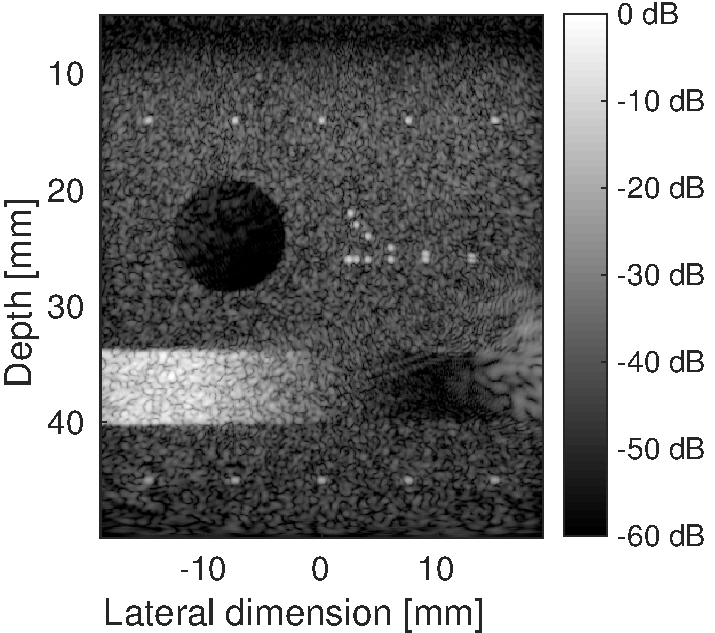
\includegraphics[width=\CohSubFigWidth]{Figures/das_dataset_rf_numerical_transmission_1_nbPW_1.pdf}}
\begin{figure}[htb]
	% Maximum length
	\hfill%
	\subcaptionbox{\label{fig_numerical_DAS}}{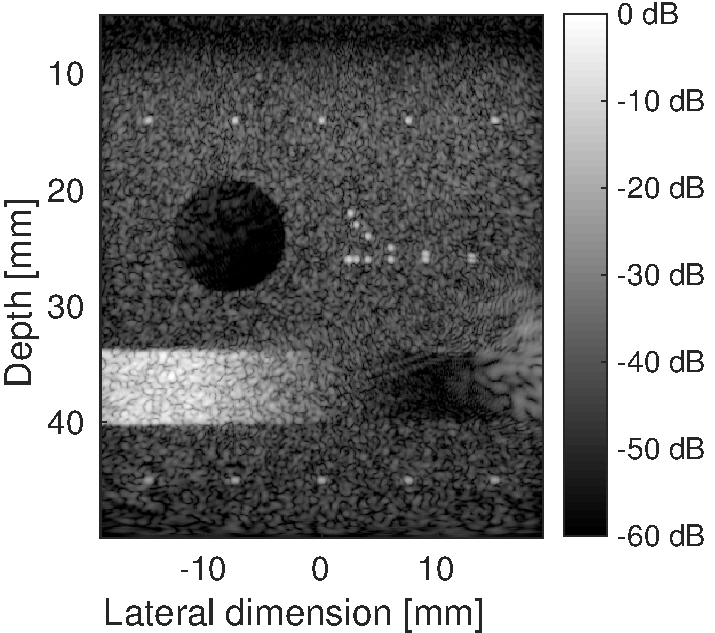
\includegraphics[height=\CohSubFigHeight]{Figures/das_dataset_rf_numerical_transmission_1_nbPW_1.pdf}}\hfill%
	\subcaptionbox{\label{fig_numerical_DAS_5}}{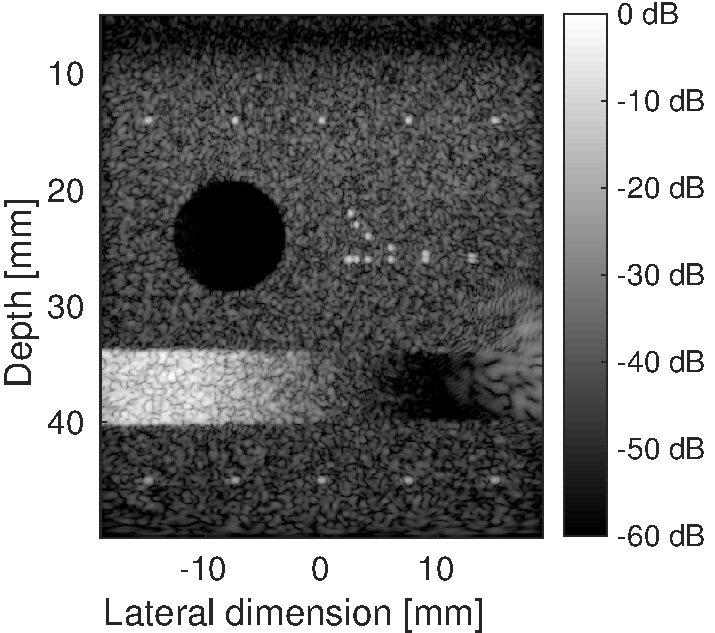
\includegraphics[height=\CohSubFigHeight]{Figures/das_dataset_rf_numerical_transmission_1_nbPW_5.pdf}}\hfill%
	\subcaptionbox{\label{fig_numerical_FISTA}}{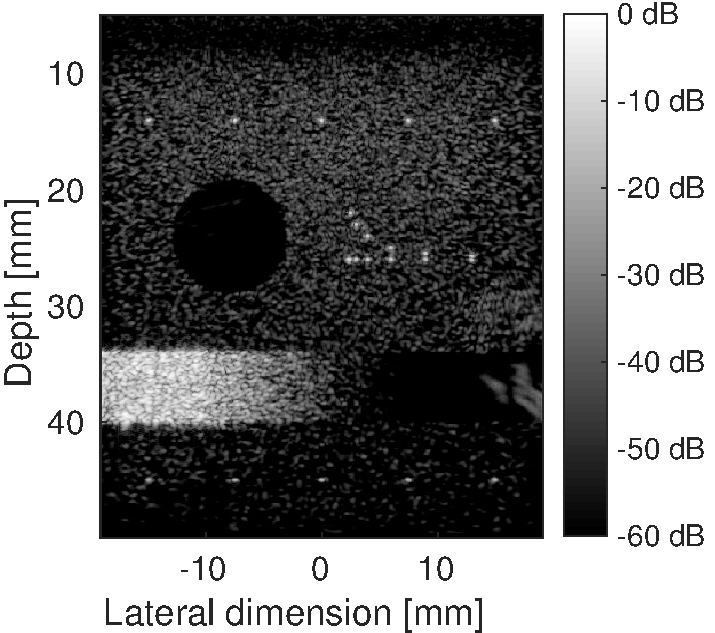
\includegraphics[height=\CohSubFigHeight]{Figures/FISTA_dataset_rf_numerical_transmission_1_nbPW_1.pdf}}\hfill%
	\subcaptionbox{\label{fig_numerical_FISTALP}}{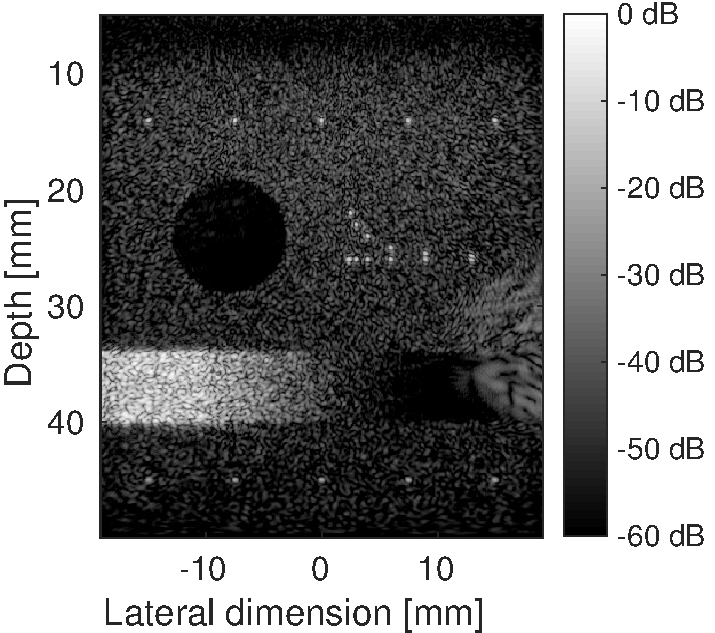
\includegraphics[height=\CohSubFigHeight]{Figures/FISTALP_dataset_rf_numerical_transmission_1_nbPW_1.pdf}}\hfill\null%
	
	\hfill%
	\subcaptionbox{\label{fig_carotid_DAS}}{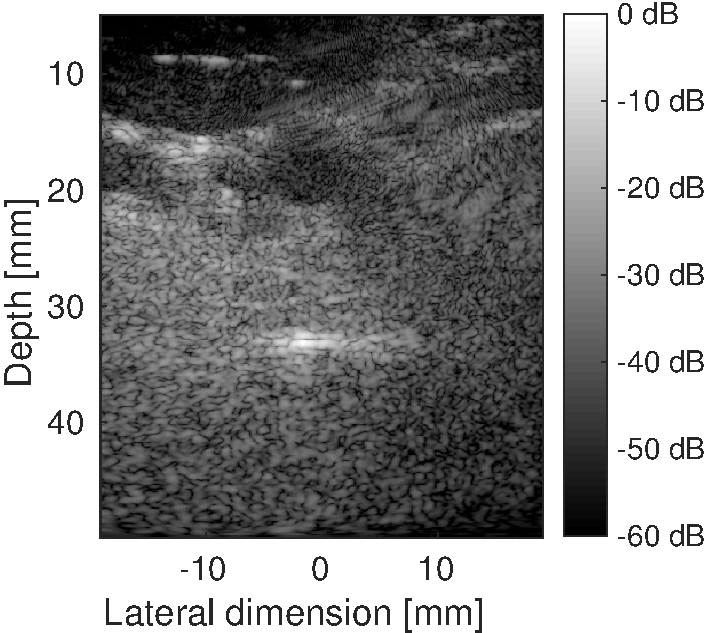
\includegraphics[height=\CohSubFigHeight]{Figures/das_carotid_cross_expe_dataset_rf_nbPW_1.pdf}}\hfill%
	\subcaptionbox{\label{fig_carotid_DAS_5}}{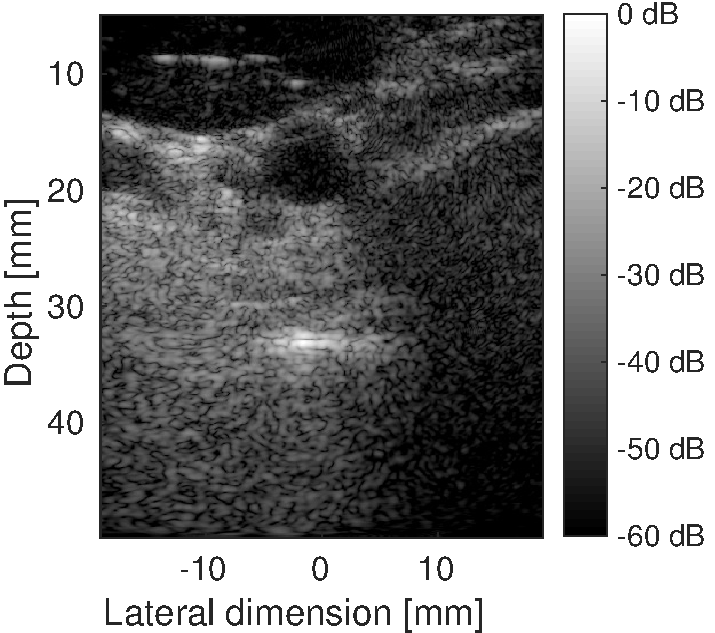
\includegraphics[height=\CohSubFigHeight]{Figures/das_carotid_cross_expe_dataset_rf_nbPW_5.pdf}}\hfill%
	\subcaptionbox{\label{fig_carotid_FISTA}}{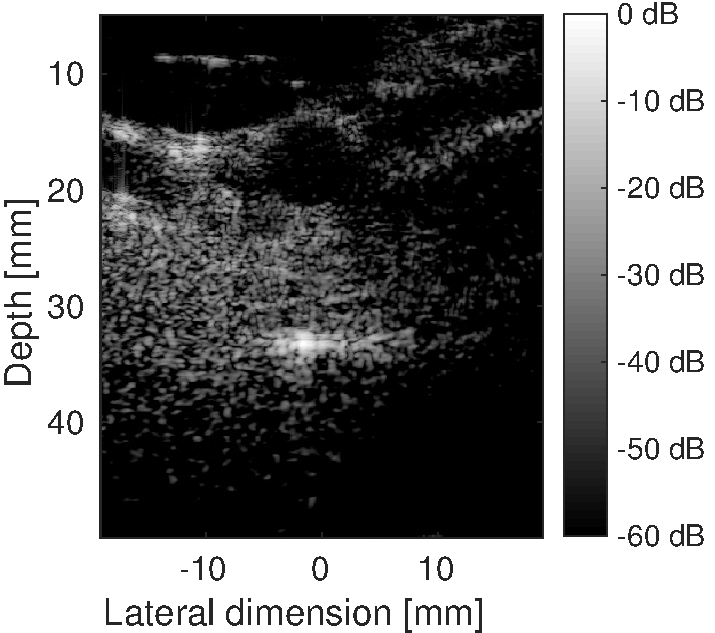
\includegraphics[height=\CohSubFigHeight]{Figures/FISTA_carotid_cross_expe_dataset_rf.pdf}}\hfill%
	\subcaptionbox{\label{fig_carotid_FISTALP}}{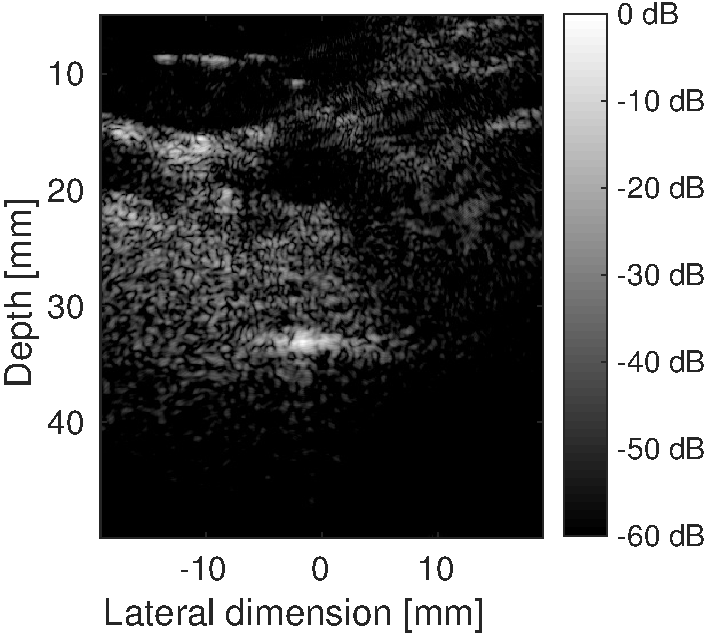
\includegraphics[height=\CohSubFigHeight]{Figures/FISTALP_carotid_cross_expe_dataset_rf.pdf}}\hfill\null%
	\caption{Image of the numerical phantom of PICMUS dataset reconstructed with (a) DAS - 1 PW insonification, (b) DAS - 5 PW insonifications, (c) USSR-SA - 1 PW insonification, (c) USSR - $\ell_p$ - 1 PW insonification; Image of the \textit{in-vivo} carotid reconstructed with (e) DAS - 1 PW insonification, (f) DAS - 5 PW insonifications, (g) USSR-SA - 1 PW insonification, (h) USSR-$\ell_p$ - 1 PW insonification.}
	\label{fig_Bmode}
\end{figure}
	
\end{block}
\vfill

%----------------------------------------------------------------------------------------
%	CONCLUSION
%----------------------------------------------------------------------------------------
\begin{block}{Conclusion and perspectives}
	\begin{enumerate}
		\item We propose USSR: an UltraSound Sparse Regularization framework
		\begin{itemize}
			\item Matrix-free and highly parallelizable formulations of measurement model and adjoint
			\item Two priors: $\ell_p$-norm in the image domain and $\ell_1$-norm in a sparsity averaging model
		\end{itemize}
		\item The proposed approach leads to high-quality at fast rates, with low-memory footprint
		\item Current work focuses on optimizing the code
	\end{enumerate}
\end{block}
\vfill
%----------------------------------------------------------------------------------------
%	BIBLIOGRAPHY
%----------------------------------------------------------------------------------------
%\begin{block}{References}
%	\printbibliography
%\end{block}
%\vfill
%----------------------------------------------------------------------------------------
%	ACKNOWLEDGMENTS
%----------------------------------------------------------------------------------------
\begin{block}{Acknowledgments}
	This work was supported in part by the UltrasoundToGo RTD project (no. 20NA21 145911), evaluated by the Swiss NSF and funded by Nano-Tera.ch with Swiss Confederation financing.
\end{block}
}%
		\end{column} % End of the second column
		
		\AddBlankColumn{\BlankColumnWidthRight} % Empty spacer column
		
	\end{columns} % End of all the columns in the poster
	
	\end{frame} % End of the enclosing frame

\end{document}

